%1521001##1##.tex
\documentclass[12pt,letterpaper]{article}
\usepackage{mathptmx}
\usepackage[margin=1in]{geometry}

\usepackage{setspace}
\doublespacing
  
\usepackage{amssymb,latexsym}
\usepackage[round,sort]{natbib}
\usepackage{fancyhdr}
\usepackage{lastpage}
\usepackage{graphicx}
\graphicspath{ {qe1/} }

% Bold Table and Figure captions
\usepackage{caption}
\captionsetup{figurename=FIGURE}
\captionsetup{tablename=TABLE}
\captionsetup[figure]{labelfont=bf}
\captionsetup[table]{labelfont=bf}
  
% Turns off all section numbering
\setcounter{secnumdepth}{0} 

  % Places all tables at end of document and creates AOM-style table-here placeholders
  \usepackage[nolists]{endfloat} % Places all figures and charts at end of manuscript and adds 'insert table x about here' lines.
  \renewcommand{\figureplace}{
    \begin{center}
    \begin{singlespace}
    ------------------------------------\\
    Insert \figurename \ \thepostfig\ about here.\\
    ------------------------------------
    \end{singlespace}
    \end{center}}
  \renewcommand{\tableplace}{%
    \begin{center}
    \begin{singlespace}
    ------------------------------------\\
    Insert \tablename \ \theposttbl\ about here.\\
    ------------------------------------
    \end{singlespace}
    \end{center}}

  \usepackage{titlesec}
   \titleformat{\title}
       {\filcenter\normalfont\bfseries\uppercase}{\thetitle}{1em}{}
  \titleformat{\section}
    {\filcenter\normalfont\bfseries\uppercase}{\thesection}{1em}{}
  \titleformat{\subsection}
    {\normalfont\bfseries}{\thesubsection}{1em}{}
  \titleformat{\subsubsection}[runin]
   {\normalfont\bfseries\slshape}{\thesubsubsection}{1em}{\hspace*{\parindent}}
       
\usepackage{tabu}
\usepackage{textcomp}
\usepackage{listings}
\usepackage{hyperref}
\usepackage{verbatim}
\usepackage{tabu}
\hypersetup{
    colorlinks=true,
    linkcolor=blue,
    filecolor=cyan,      
    urlcolor=cyan,
    citecolor=blue,
}

\usepackage{etoolbox}

\makeatletter

% Patch case where name and year are separated by aysep
\patchcmd{\NAT@citex}
  {\@citea\NAT@hyper@{%
     \NAT@nmfmt{\NAT@nm}%
     \hyper@natlinkbreak{\NAT@aysep\NAT@spacechar}{\@citeb\@extra@b@citeb}%
     \NAT@date}}
  {\@citea\NAT@nmfmt{\NAT@nm}%
   \NAT@aysep\NAT@spacechar\NAT@hyper@{\NAT@date}}{}{}

% Patch case where name and year are separated by opening bracket
\patchcmd{\NAT@citex}
  {\@citea\NAT@hyper@{%
     \NAT@nmfmt{\NAT@nm}%
     \hyper@natlinkbreak{\NAT@spacechar\NAT@@open\if*#1*\else#1\NAT@spacechar\fi}%
       {\@citeb\@extra@b@citeb}%
     \NAT@date}}
  {\@citea\NAT@nmfmt{\NAT@nm}%
   \NAT@spacechar\NAT@@open\if*#1*\else#1\NAT@spacechar\fi\NAT@hyper@{\NAT@date}}
  {}{}

\lstset{
basicstyle=\ttfamily,
columns=flexible,
breaklines=true
}
\newenvironment{hypothesis}{
  	\itshape
  	\leftskip=\parindent \rightskip=\parindent
  	\noindent\ignorespaces}

\fancypagestyle{plain}{
  \renewcommand{\headrulewidth}{0pt}
  \fancyhf{}
}	


\begin{document}
\title{Title: Sub-title}
\date{}
\maketitle

\begin{abstract} 
\normalsize 
We apply a formal model to understand the effects of the relative learning rates of embedded agents and the institutional field on organizational outcomes. 
\end{abstract}


{\textbf{Keywords:} \\\indent Embedded Agency}

\newpage
\pagestyle{fancy}
\fancyhf{}
\lhead{Title}
\rhead{\thepage}

\begin{center}
\textbf{Title: Sub-title}
\end{center}
Our understanding of  institutional phenomena has come a long way since \cite{Selznick1957} made the observation that organizations adopted new goals suited to existing structures  instead of changing the structures that may have outlived their utility. 

The rest of this article is organized as follows. 

\section{Background}
 \cite{Scott1995} visualized institutional fields as a community of organizations that partakes of a common meaning system and whose participants interact more frequently and fatefully with one another than with actors outside the field. 
 
\section{Model}

We develop a simple model consisting of two players who participate in a repeated game of matching \footnote{I am grateful to Phanish Puranam for having introduced me to this model of reinforcement learning during a workshop at the Indian Institute of Science on 16th December, 2016. His definitions and code have been extensively reused in this work.}. The payoffs are captured by the matrix in Table ~\ref{payoffmatrix}

\begin{table}
\begin{centering}
\caption {Payoff Matrix}
\label{payoffmatrix}
{\tabulinesep=1.4mm
\begin{tabu}{|c|c|c|}
\hline
&$choice_F(t) = 0$&$choice_F(t) = 1$\\\hline
$choice_A(t) = 0$&$[payoff_F(t),payoff_A(t)]=[1,1]$&$[payoff_F(t),payoff_A(t)]=[0,0]$\\\hline
$choice_A(t) = 1$&$[payoff_F(t),payoff_A(t)]=[0,0]$&$[payoff_F(t),payoff_A(t)]=[1,1]$\\\hline
\end{tabu}}

\end{centering}
\end{table} 

To help improve the intuition in the analysis, we define a few categories. 

\subsection{Field Start Position}
The Field Start Position is a characterization of the choice preference of the institutional field at the start of the interaction. 
\subsubsection{The third level section}
We do so since the scale is symmetric across the Center (C), any initial mapping of Left (L) and Left of Center (LC) can be mapped onto an equivalent Right (R) or Right of Center (RC) configuration. 

\begin{figure}[h]
\begin{centering}
  \caption{}
  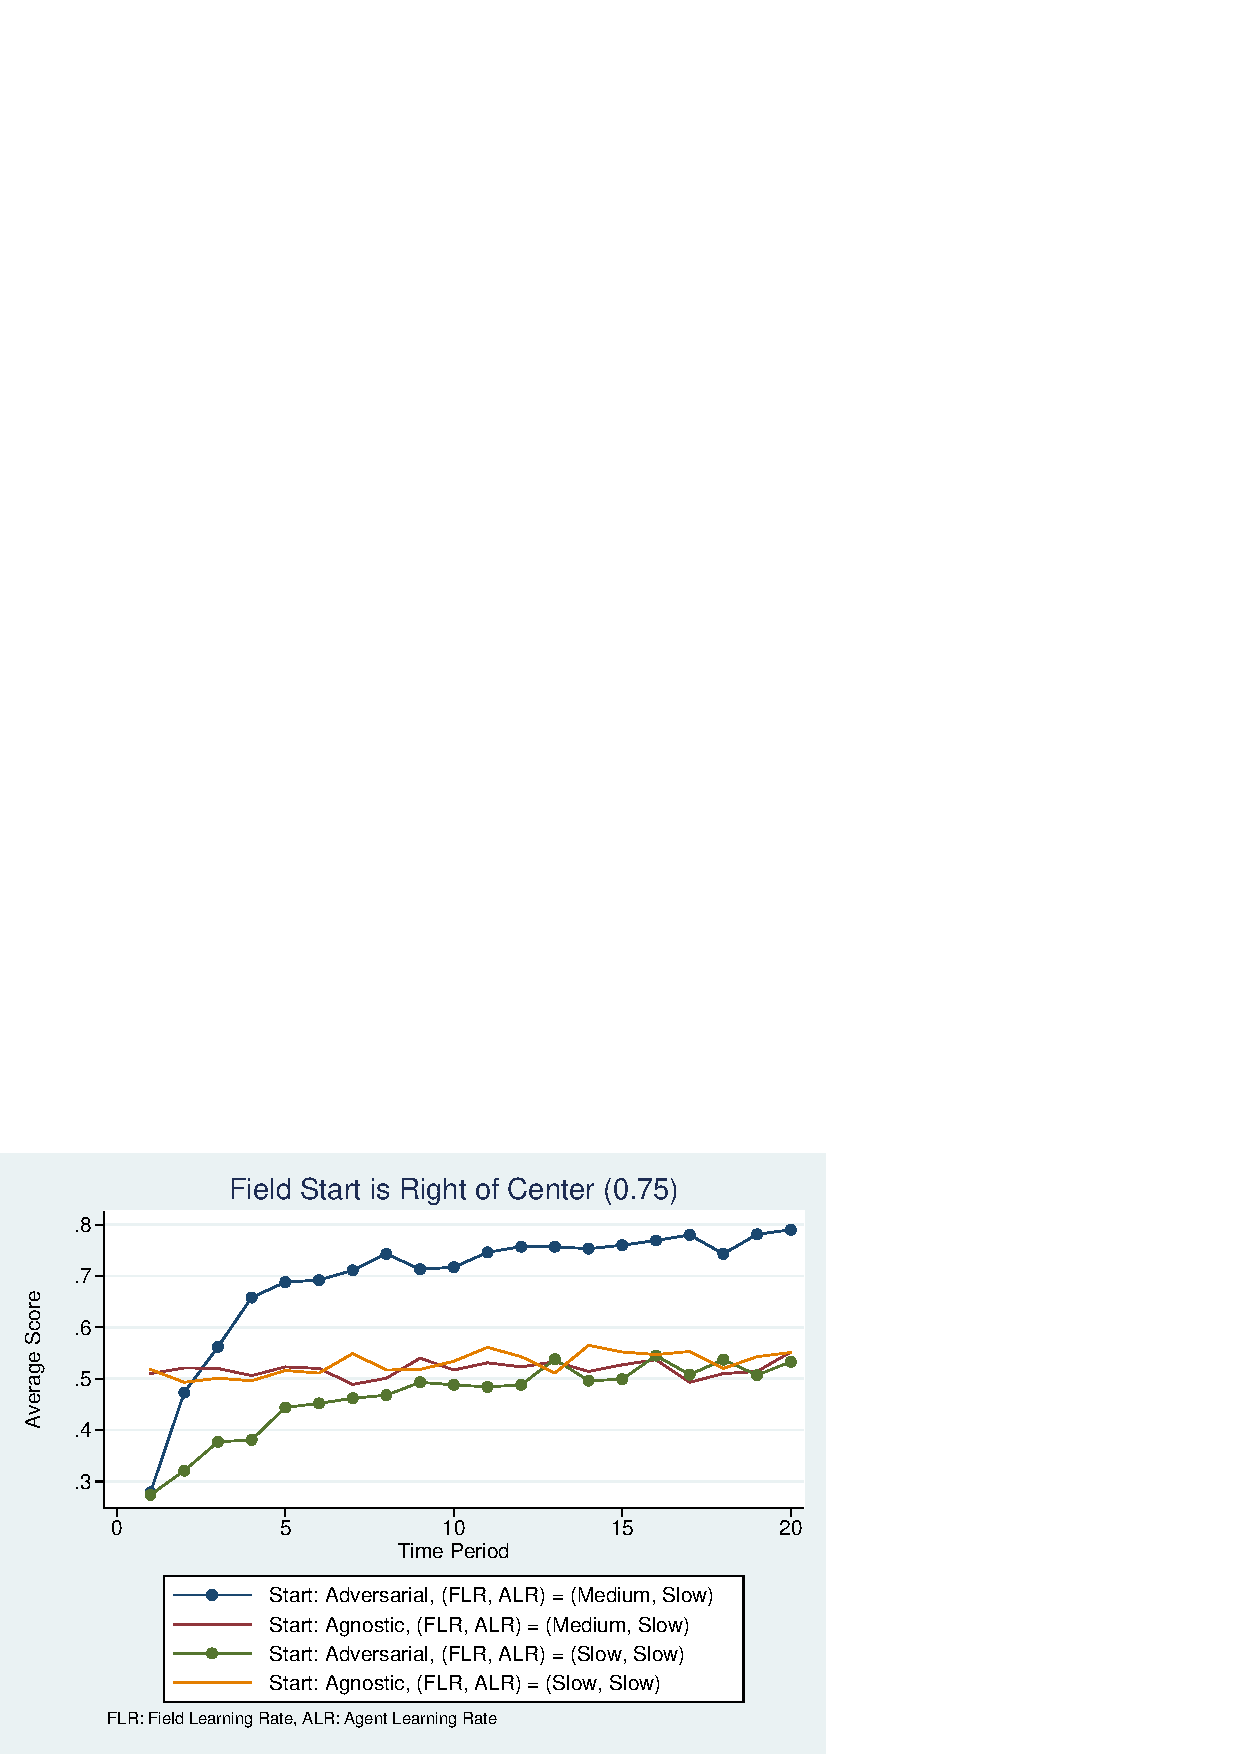
\includegraphics[width=\textwidth]{frcmedium3a}
  \label{fig:3a}
\end{centering}
\end{figure}

\section{Discussion}
Having laid out the formal model and having described the assumptions and classifications made in the previous section, we now consider if the model described above is a reasonable abstraction of the phenomenon that we wish to theorize upon. 

\section{Interpretation of Model Results}
\subsection{On the topic of the general hypotheses}
 Figure ~\ref{fig:3a} lays out the average score charts for four agent-field combinations while enforcing the field to start in Right of Center (this is the same as saying $p_{0,F}^0 = 0.75$). 
\subsubsection{Leading into H1a}
We do so since the scale is symmetric across the Center (C), any initial mapping 

\begin{hypothesis}
{Hypothesis 1a: When the institutional field is open to influence, slow learning adversarial agents will raise overall performance higher than slow learning agents with a neutral orientation\\}
\end{hypothesis}

\subsubsection{Leading into H2a}
This trend is confirmed further in Figure ~\ref{fig:3a} where the learning rates of agents are increased even further to \textquotesingle Fast\textquotesingle .

\begin{hypothesis}
{Hypothesis 2a: For the same initial outcome preferences,  the overall performance score varies curvilinearly with difference in the rates of learning of the agent and the institutional field\\}
\end{hypothesis}

\section{Limitations and Future Work}
The formal computational modeling approach to theorizing organizational phenomena comes across as being both valuable and challenging simultaneously. 


\section{Conclusion}
We started out attempting to improve our understanding of the mechanisms behind the embedded agent - institutional field engagement. 

\begin{comment}
\section{Acknowledgements}
All mistakes made here are completely mine. 
\end{comment}

\newpage
\begin{singlespace}
\bibliography{/Users/aiyenggar/code/bibliography/aiyenggar} 
\bibliographystyle{ai-amjlike}
\end{singlespace}

\newpage
\appendix
\begin{singlespace}
\section{APPENDIX A: Simulation Code}
\lstinputlisting{qe1/matchingEmbeddedAgency.py}
\end{singlespace}

\end{document}
